\section{Introduction}
% Traditional research on social science
Social science investigates human behavior and social structures to understand how societies function. Traditional sociological research heavily relies on human participation to conduct experiments and gather data. Questionnaires~\cite{granovetter1973strength,katz2015social} and psychological experiments~\cite{asch1951effects,milgram1963behavioral} are commonly used to test theoretical hypotheses, understand social phenomena, and predict collective outcomes. While these methods can provide highly authentic data, they are expensive, challenging to scale, and involve certain ethical risks.

Recently, large language models (LLMs) have demonstrated impressive capabilities in human-level reasoning and planning~\cite{wei2022chain,kojima2022large,xi2023rise,yao2024tree,Wang_2024}. They can perceive the environment, make decisions, and take corresponding actions, showcasing their potential as autonomous agents that can serve as human substitutes. In appropriate settings, LLM-driven agents can accurately simulate responses from corresponding individuals by leveraging their role-playing abilities~\cite{shao2023characterllmtrainableagentroleplaying,chen2024persona}, a property known as algorithmic fidelity~\cite{Argyle_2023,chaudhary2024large}. This characteristic makes LLM-driven agents highly valuable in simulating human behavior. By reproducing individual response patterns in specific scenarios, LLM-driven agents help researchers to better understand, validate, and predict human reactions.

\begin{figure*}[!t]
    \centering
    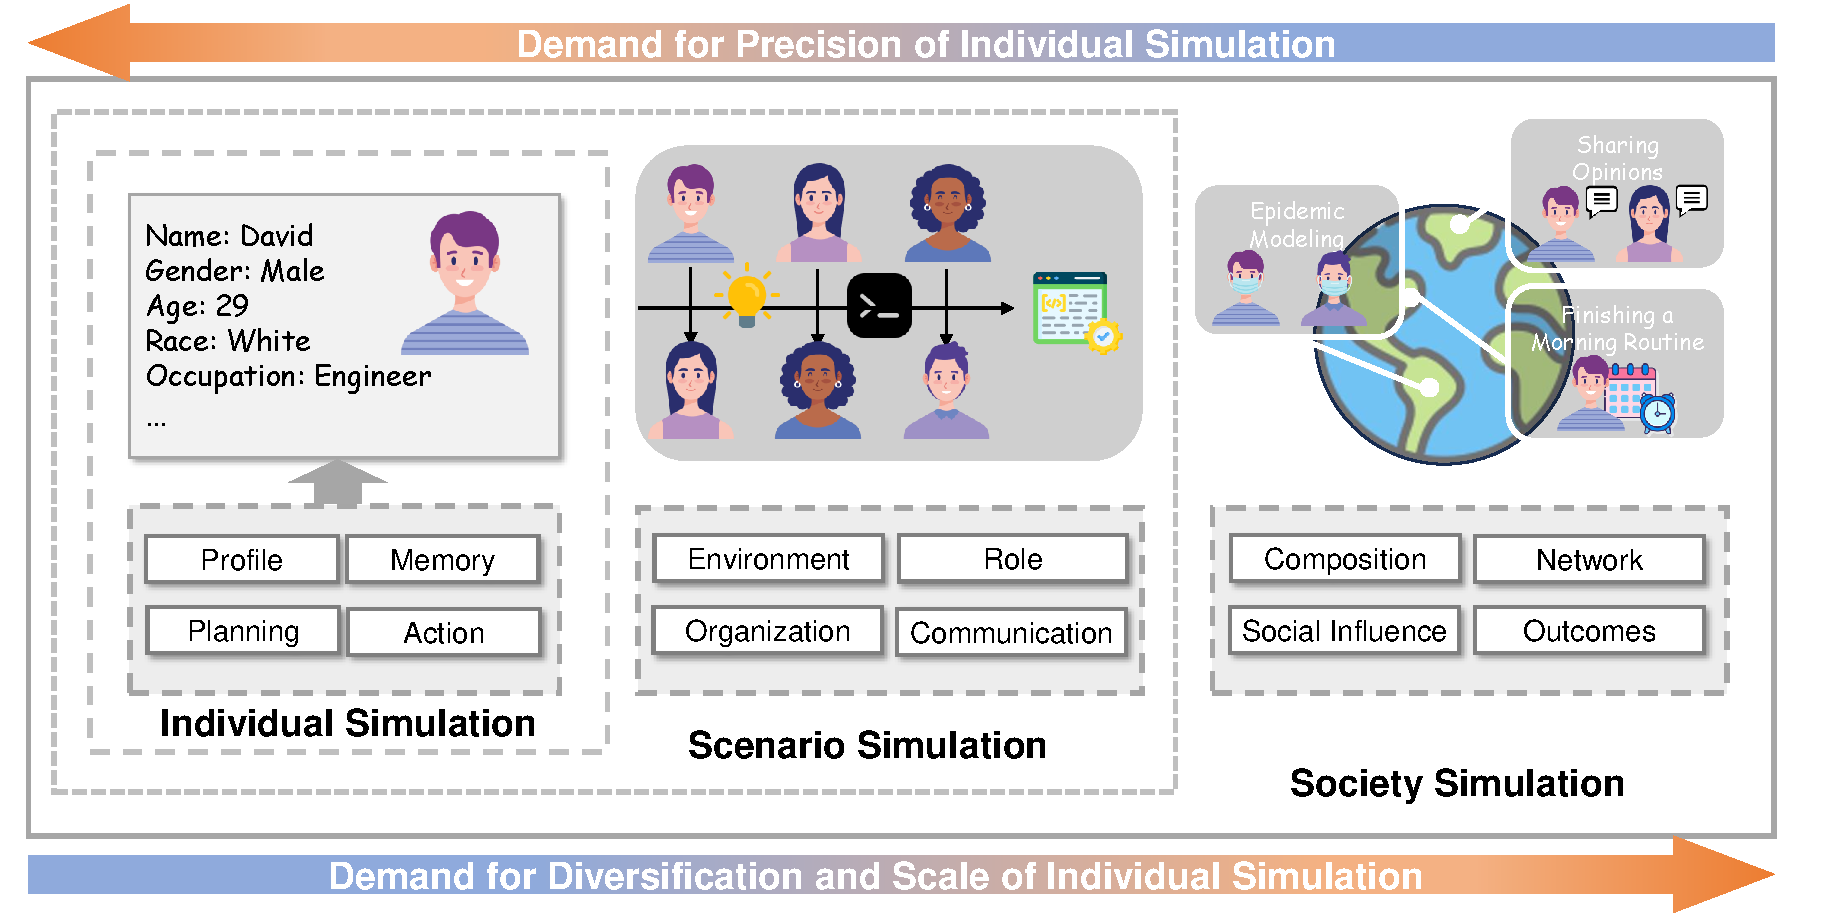
\includegraphics[width=\linewidth]{figs/intro.pdf}
    \caption{Illustration of simulations empowered by LLM-driven agents. We categorize the simulations into individual simulation, scenario simulation and society simulation. From left to right, the diversity and scale of individual modeling generally increase. Conversely, from right to left, the granularity of individual modeling becomes more refined.}
    \label{fig:intro}
\end{figure*}

Just as individuals do not exist independently within society, in addition to separate individual agents, interactions between multiple agents have also been widely studied to solve specific problems or simulate complex dynamics in the real world~\cite{guo2024large,gao2024large}. On one hand, LLMs can be specialized as agents with detailed knowledge and skills, leveraging collective intelligence to solve complex problems, such as software development~\cite{qian2023communicative,hong2023metagpt}, automatic diagnosis~\cite{li2024agent,fan2024ai} and judicial decision-making~\cite{he2024simucourt}. In this case, multiple autonomous agents collaborate on planning, discussion, and decision-making, reflecting the cooperative nature of human groups when solving problems. On the other hand, simple interactions between multiple agents can lead to the emergence of complex collective behaviors or patterns~\cite{schelling1971dynamic,hegselmann2005opinion,chuang2023computational}, thereby replicating complex social dynamics in the real world, such as opinion dynamics~\cite{chuang2023simulating,mou2024unveiling,liu2024skepticism} and macroeconomics phenomena~\cite{li2024econagent}.  Such simulations provide valuable tools for understanding, analyzing, and predicting complex phenomena that may be difficult or impractical to observe directly in real life, offering strong support for decision-making in areas such as policy-making and social management.

This research field is rapidly expanding, with papers focusing on various aspects. Considering the purpose of simulation and the varying demands for diversity, scale, and accuracy in individual modeling, we categorize the existing work into three types, as illustrated in Figure~\ref{fig:intro}: 

\begin{enumerate}
    \item \textbf{Individual Simulation}: leveraging LLM-based agents to mimic specific individuals or groups of people sharing common demographic characteristics~\cite{wang2024rolellmbenchmarkingelicitingenhancing,shao2023characterllmtrainableagentroleplaying,chen2024persona}. This line of research focuses on the replication of features of a single person, e.g., personality, and has not involved multi-agent interactions.
    
    \item \textbf{Scenario Simulation}: organizing a group of agents in a concentrated scenario, driven by specific goals or tasks, such as software development~\cite{qian2023communicative,hong2023metagpt}, question answering~\cite{du2023improving} and paper reviewing~\cite{d2024marg}. Such simulations are usually focused on small-scale agents within specific scenarios,  emphasizing the collective wisdom of agents with specialized expertise.
    
    \item \textbf{Society Simulation}: simulating more complex and diverse behaviors in the agent society to explore social dynamics in real-world applications. Such simulations could test social science theories within a small scope~\cite{chuang2024wisdom} or populate virtual spaces and communities with large-scale realistic social phenomena~\cite{park2023generative,yang2024oasis}. The composition of individuals in such simulations is more complex and diverse.
\end{enumerate}

These three types of simulations exhibit a progressive relationship. Individual simulation models a specific person or a type of person, serving as the foundation for scenario simulation and society simulation. Theoretically, society simulation can encompass a chaotic world composed of countless sub-scenarios, though current work focuses on specific scenarios.

Although this field has seen rapid growth, with some surveys summarizing agent architectures~\cite{xi2023rise,Wang_2024,gao2024large} or certain aspects of single-agent ability or multi-agent systems~\cite{chen2024persona,guo2024large,liu2024large}, there is an absence of a systematic review to summarize the work from the individual to society, providing a comprehensive blueprint for this field. This motivates us to present this survey, aiming to contribute to the research and development of simulations driven by LLM-based agents, as well as a wider range of interdisciplinary studies. To comprehensively describe our landscape, we organize our survey as follows. After a brief introduction to the background in ~\S~\ref{sec:bg}, we begin in ~\S~\ref{sec:indi} by detailing how to conduct individual simulation through discussions of (1) the architecture of a single agent, (2) construction method of individual simulation, (3) the classification of objectives, and (4) the evaluation of individual simulation. Next, in ~\S~\ref{sec:task}, we summarize scenario simulation, including (1) the elements that constitute a scenario simulation system, (2) the classification of scenarios, and (3) the evaluation of scenario simulation, exploring how multiple agents collaborate to achieve objectives within a single scenario. Following this, in ~\S~\ref{sec:soc}, we introduce society simulation, examining how multi-agent systems can construct complex social dynamics through (1) the social construction elements of society simulation, (2) the classification of society simulation scenarios, and (3) the evaluation of society simulation. In ~\S~\ref{sec:data}, we summarize existing datasets and benchmarks. Based on the earlier sections, we analyze trends in these three aspects in ~\S~\ref{sec:trend} and present the conclusion in ~\S~\ref{sec:con}.

\begin{figure*}[t]
    \centering
    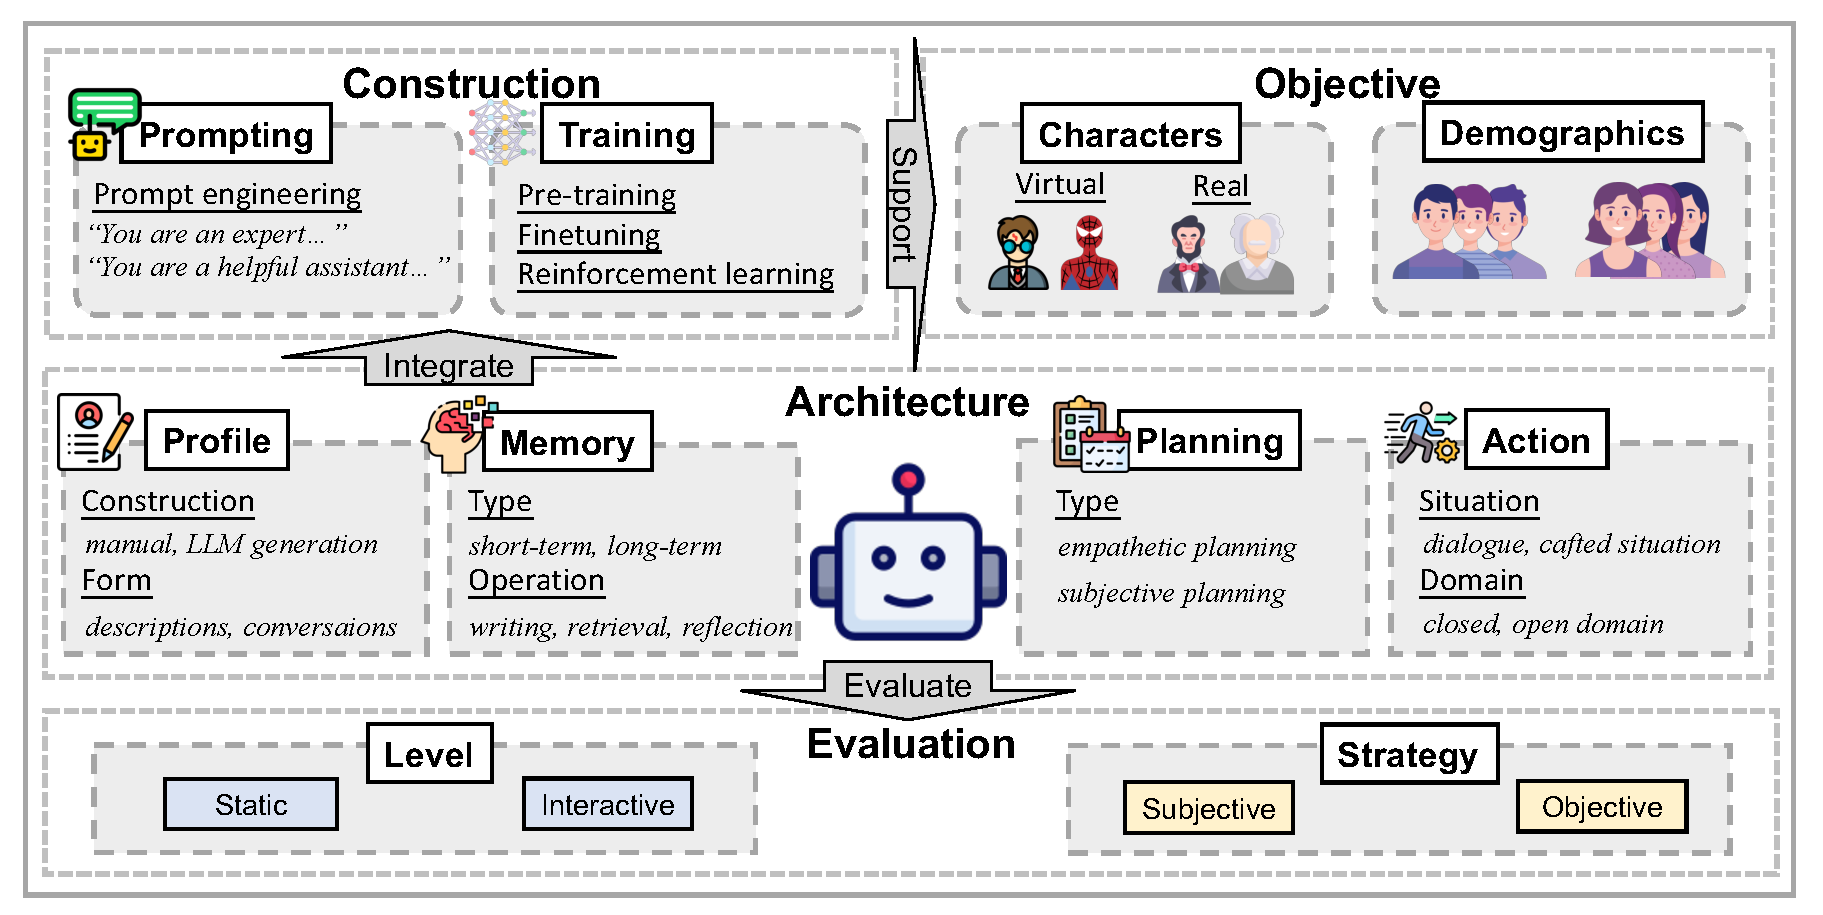
\includegraphics[width=\linewidth]{figs/fm_indi_v2.2.pdf}
    \caption{Illustration of individual simulation blueprint. An individual agent is typically composed of an {\ul architecture} with modules involving profile, memory, planning, and action through  {\ul construction} method, prompting or training, to simulate specific {\ul objectives} like characters or demographics . Individual simulation can be {\ul evaluated} statically and interactively with different dimensions being observed.}
    \label{fig:fm_indi}
\end{figure*}

\section{Background}~\label{sec:bg}
\subsection{Large Language Model-based Agents}
Benefiting from the large-scale parameters and pre-training on vast amounts of data, the recently emerging large language models have shown great potential in achieving human-like intelligence~\cite{brown2020language,kojima2022large,achiam2023gpt}. This has sparked a rise in the research of LLM-empowered agents, where the key idea is to equip the LLMs with human capabilities such as memory~\cite{fischer2023reflective,wang2023user}, planning~\cite{yao2022react,hao2023reasoning} and tool usage~\cite{parisi2022talm,schick2024toolformer}. The memory module enables agents to store and operate historical information to facilitate future actions. Memory of different structures~\cite{park2023generative,shinn2024reflexion} and formats~\cite{hu2023chatdb,zhong2024memorybank} have been integrated into LLM-based agents. The planning module helps agents to decompose complex tasks into subtasks, where various planning strategies~\cite{wei2022chain,yao2022react} are adopted. The tool-usage module allows agents to make use of external tools or resources~\cite{yao2022react,ruan2023tptu} to solve tasks. Overall, these modules assist agents in operating more effectively in complex and diverse environments.

\subsection{Multi-agent Systems}
To realize complex scenarios, a single agent is never enough. A system where interaction between multiple agents is involved is referred to as a multi-agent system (MAS). The agents may have a common goal, such as working together to accomplish a task~\cite{qian2023communicative,hong2023metagpt} or solve a problem~\cite{du2023improving}, or they may just have self-interested goals that can cause them to compete for limited resources~\cite{hua2023war}. In a multi-agent system, each agent may be assigned distinct roles and skills, as well as distinct tasks. These agents can be organized in various ways, such as layered or centralized structures~\cite{qian2024scaling,hao2023chatllm,li2024culturepark}, and can communicate through different methods~\cite{chen2024beyond,phamlet,marro2024scalable}. These factors significantly influence the effectiveness and efficiency of multi-agent interactions.


% Researchers have focused on different aspects of the systems, such as organization~\cite{qian2024scaling} and communication~\cite{phamlet,chen2024beyond} to improve the system's performance. 





